\section{Deployment view (UML Deployment diagram)}\label{sec:deployment}

\begin{sidewaysfigure}[!htp]
    \centering
    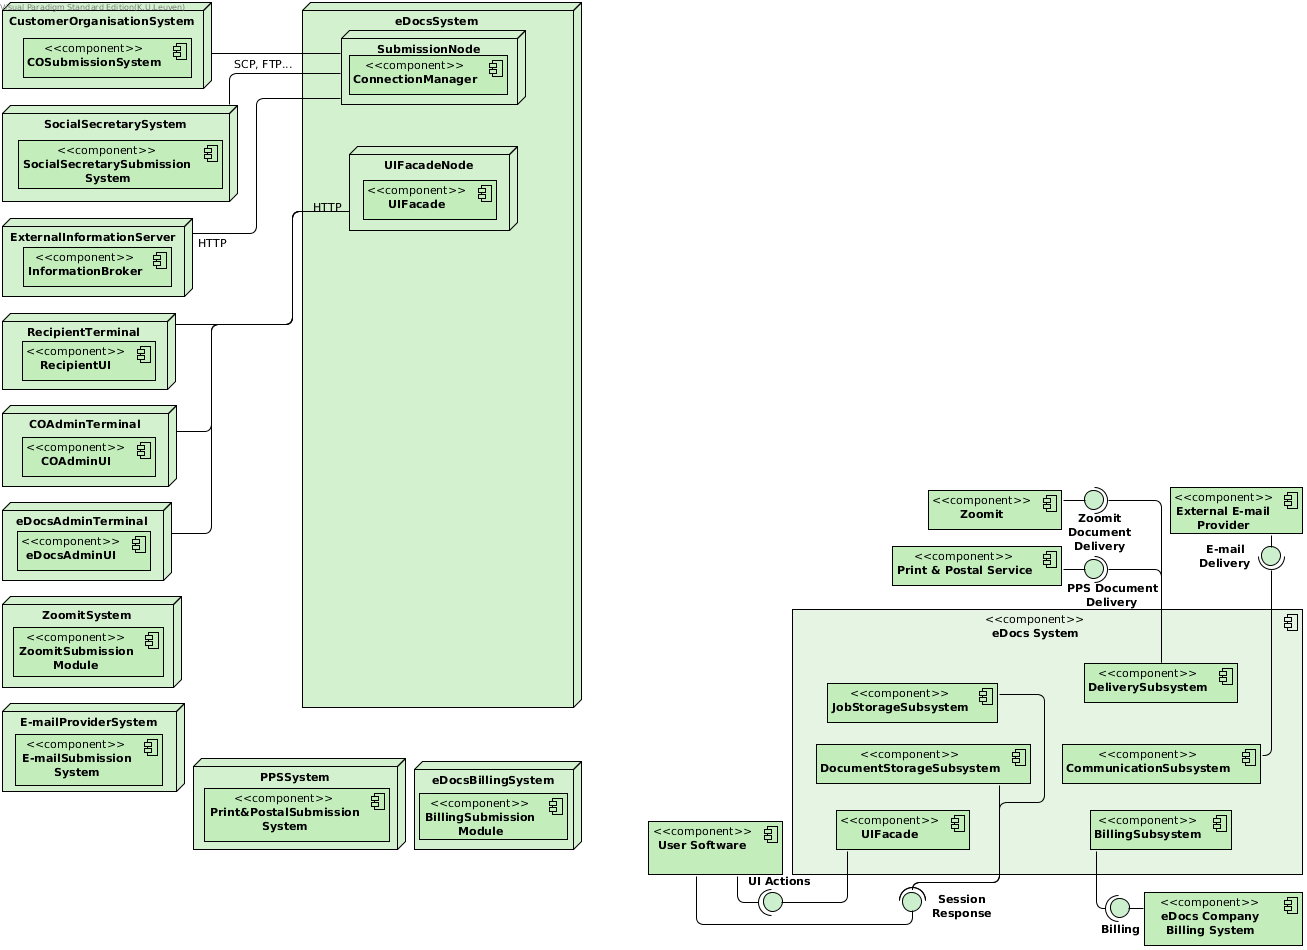
\includegraphics[width=0.8\textwidth]{figures/Deployment Context.png}
    \caption{Context diagram for the deployment view.}\label{fig:depl_context}
\end{sidewaysfigure}

Figure \ref{fig:depl_context} shows the Context Diagram for the deployment of the system.\\
The \ttt{SubmissionSubsystem} is contacted for Raw Data Submission over FTP, SCP, etc. as stipulated in the SLA (conform the initial description). It also connects to an \ttt{InformationBroker} over HTTP to lookup information for consistency checks of Raw Data.\\
The different types of UI's (the \ttt{RecipientUI}, \ttt{COAdminUI} and \ttt{eDocsAdminUI}) connect to the UIFacade through the HTTP protocol, be it via a web browser or a user application. The response from a user's session is delivered back by the UIFacade (more precisely by the session of the user on the serverside) over the same protocol.\\
The \ttt{DeliveryChannels} send documents to their respective services over the protocol as stipulated by the service (FTP,SCP,...).\\
Nodes from the \ttt{CommunicationSubsystem} use SMTP to send e-mails via the \ttt{E-mailSubmissionSystem}, and the \ttt{ExternalNotificationAcceptor} also receives messages over SMTP from e.g. Zoomit or the e-mail provider (in case of failures, deliveries...).\\
The \ttt{BillingSubsystem} interfaces with an external billing system of the eDocs company through a general (FTP,SCP...) protocol to process billing to Customer Organisations.

\begin{figure}[!htp]
    \centering
    %\includegraphics[width=\textwidth]{}
    \missingfigure[figwidth=0.8\textwidth]{Primary diagram for the deployment
        view.}
    \caption{Primary diagram for the deployment view.}\label{fig:depl_primary}
\end{figure}


Figure \ref{fig:depl_primary}. The primary deployment diagram itself and accompanying explanation.
Pay attention to the parts of the deployment diagram which are crucial for
achieving certain non-functional requirements.
Also discuss any alternative deployments that you considered.